\documentclass[10pt,draftclsnofoot,onecolumn,journal,compsoc]{IEEEtran}


\setlength{\parindent}{0em}
\setlength{\parskip}{1em}



\usepackage[margin=0.75in]{geometry}
\geometry{textheight=9.5in, textwidth=7in}
\usepackage{listings}
\usepackage{comment}
\usepackage{imakeidx}
\usepackage{graphicx}
\usepackage{float}
\usepackage{listings}
\usepackage{url}
\usepackage{longtable}
\usepackage{enumitem}
\usepackage{setspace}
\singlespacing


\def \DocType{		%Problem Statement
	%Requirements Document
	%Technology Review
	Design Document
	%Progress Report
}



\lstset{
  basicstyle=\small\ttfamily,
 numbers=left,
  numberstyle=\scriptsize,
  showspaces=false,
  showstringspaces=false,
  breaklines=true
}





% 1. Fill in these details
\def \CapstoneTeamName{DSCVL-Overcomers}
\def \CapstoneTeamNumber{69}
%\def \GroupMemberOne{KIN-HO LAM}
\def \GroupMemberTwo{LUCIEN-ARMAND T. TAMNO}
%\def \GroupMemberThree{			}
\def \CapstoneProjectName{Depth sensing with computer vision and lidar }
\def \CapstoneSponsorCompany{}
\def \CapstoneSponsorPerson{ D. Kevin McGrath}

\usepackage{datetime}
\newdate{date}{19}{3}{2018}
\date{\displaydate{date}}

\title{\centering
			
\includegraphics[height=4cm,natwidth=200,natheight=300]{images/osu_logo.png}\\\vspace{.5in}
		\scshape{\huge CS CAPSTONE \DocType \\\vspace{.5in}
		\textbf{\Huge\CapstoneProjectName}\\\vspace{1in}
		\large	\displaydate{date}\\\vspace{.3in}		
			\large {Prepared For}\\\vspace{.1in}
			\textbf{{\Large \CapstoneSponsorPerson}} \\\vspace{.8in}		
				\large {By} \\\vspace{.1in}
				\textbf {Group \CapstoneTeamNumber}\\\vspace{.1in}
				\large {\CapstoneTeamName}\\\vspace{.1in}
				\textbf{ { \GroupMemberTwo}}
}  
}

\IEEEtitleabstractindextext{

 \begin{abstract}
Depth sensing using computer vision and lidar project on this its winter progress report is to elaborate on its purpose, to detail on current stage, the dynamic ofits members as well as the history of the work done.
 \end{abstract} 
 

}
%%%%%%%%%%%%%%%%%%%%%%%%%%%%%%%%%%%%%%%

\begin{document}
\pagenumbering{gobble}
 \maketitle
\IEEEdisplaynontitleabstractindextext
\IEEEpeerreviewmaketitle
\newpage
\pagenumbering{arabic}
\tableofcontents
\newpage
	
\section{Table of Contents}
\tableofcontents
\bibliographystyle{IEEEtran}


\begin{singlespace}
	\section{Definitions}
			\textbf{IR: }\label{def:IR}\par
		IR stands for the infrared technology.

		\textbf{IR Depth Sensor: }\label{def:depthsensor}\par
		A device that calculates distances by emitting infrared signals. 
		
		\textbf{LIDAR: }\label{def:lidar}\par
		Light Detection And Ranging - A method that uses lasers to measure distance
		
		\textbf{Microsoft Kinect: }\label{def:kinect}\par
		A product that uses an IR Depth sensor to measure distances.
		
		\textbf{Logitech Brio Webcam: }\label{def:brio}\par
		The webcam model this project shall be using.
		
		\textbf{RPLidar A1: }\label{def:rplidar}[1]\par
		A low-cost LIDAR unit that this project shall be using.
		
		\textbf{RPLidar Solid-state: }\label{def:rplidar2}[2]\par
		A High-cost LIDAR unit single direction with better performances of detecting, measuring and locating liquids and people
		
		\textbf{Computer Vision: }\label{def:vision}\par
		The methods for acquiring, processing, analyzing, and classifying digital images and extracting information.
		
		\textbf{GUI: }\label{def:gui}[3]\par
		GUI: Graphical User Interface
		
		\textbf{Videocapture: }\label{def:videocapture}[4]\par
		videocapture: Stream of subsequent images
		
		\textbf{DSCVL: }\label{def:DSCVL}\par
		Acronym that stands for Depth sensing with computer vision and lidar


		
		
	\section{Project Purpose}
The purpose of the DSCVL project is to come up with an effective solution that is to paint an overlay image with a single point signal both from different kinds of technology. In fact, the solution uses the Lidar technology ( the solid-state rplidar) that shows better performance in the outdoor environment when is to detect, locate, and measure objects   including liquids and people by using sensors pulsing laser to reach its subject and does that with great accuracy than the infrared-based technology can do. For the IR though seems to provide exact measurements in the indoor environment, on the other hand, performs poorly outside. The second technology using the a camera in this case, the Logitech Brio Webcam would capture video stream to turn into images that would be combined to the point lidar points output. And finally, This entire process   would equip the  stakeholder specially the client of the DSCVL project with a tool to trace movements, see any subject of interest and precisely determine the distance of which the subject of interest is found.	


\section{Current State}
At the current stage,though the application to implement has not yet reached its ultimate goal that is to put in display an overlay image as required by the client, nonetheless i was able during the past ten weeks to do the following tasks:

\subsection{Progress- the project frontend}
The first place i got started was to write user python-based interface using what was for me a relevant python library known as the "appJar" library. However, over the course of the implementation, i ran into the issue of the documentation to keep on  working with appJar library to write some needed functions such as the events handlers routines. And that set me into a path to look for another library, in this case the tkinter library. And currently, this is the GUI i got ( see figure 1).\\
    	\begin{figure}[ht]
    	 \centering 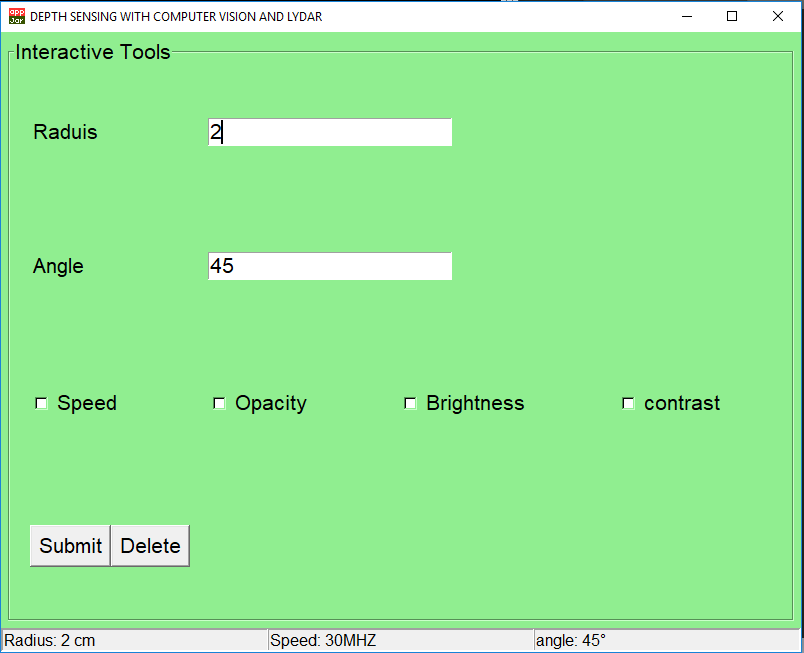
\includegraphics[width=4.5in,natwidth=4000,natheight=200]{images/userinterface.png}
    	\caption{figure}{ Graphical user interface, python-based implimentation}\label{def:gui}
    	\end{figure}
    	
Afterward, i switched back and got involved in the backend of the project.

	\subsection{Progress-the project backend}
the part of the project, i am called to work in consist of writing functions to get data receive from the rplidar for example the rplidar A1 and change those data to be useful information to trace and  locate with precision any subject that the user could be interesting found within the application boundaries of computation. so far, i have written functions that allow to transform  rplidar device string of characters onto an array of values, another function to receive as input the previous array, compute and return another array of values providing the various angles as the subject moves along the Z-axis, and i can display data as shown by the following figure2:
\begin{figure}[ht]
    	 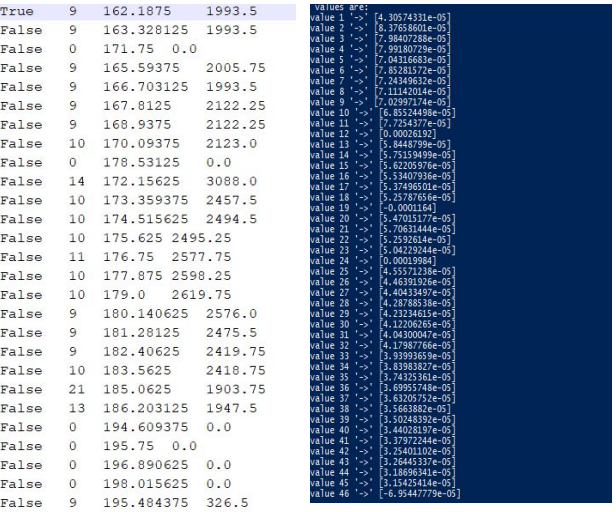
\includegraphics[width=6in,natwidth=2000,natheight=200]{images/output.png}
    	\caption{figure}{ data from the rplidar scanner device(leftside) \& outcomes from dynamic object function (rightside) of the figure}
    	\end{figure}
    	
    	\textbf{\textit{Associate code of execution of the above figure}•}
    	
    	this code is a snippet code that describes how data  are processed. 
    	
    	\begin{figure}[ht]
    	\centering
    	 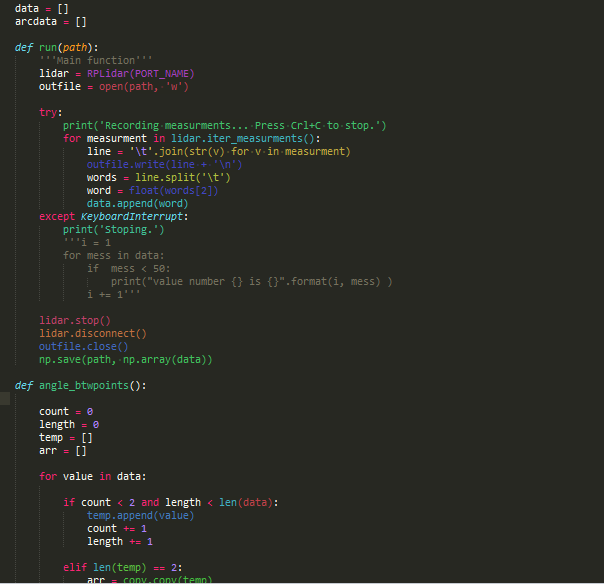
\includegraphics[width=4.5in,natwidth=2000,natheight=100]{images/snapcode.png}
    	\caption{figure}{  python-based code of execution}
    	\end{figure}
    
   \pagebreak 
   	
Additionally, having in mind that our application has to run on multiple plaforms namely Windows, MacOS and Linux, we are simultaneously  writing this application on Windows and Linux, and interchangeably tools from either of the  platforms mentioned above. 
I am Saying we is to mean, Lam and who work on the project.		
	
	\subsection{Group Evaluation}
		My teammate Lam, beyond the fact of being a hardworking guy, an excellent communicator, has an impressive skill of an organizer. From day one, Lam is committed himself to the project, engaging to it day in day out.
		under Lam leadership and in almost eight weeks, we have relentlessly pushed  boundaries, he always reviews and explores new of ways that could grant us the pathway to final solution.   project.
		though, we have not yet  reached the ultimate goal which is who have to have the overlay, paint image on the screen, Lam optimist, engagement, excellent work ethic and enthusiasm, self determination are all solid signs  that demonstrate that our project will get into its final stage.
		Honestly, Lam is a great teammate to work with and in the workplace if he keep on  working and displaying all the skills mentioned above, that will not be surprising to see him leading people. 
		
	Just to elaborate a little bit on Lam character, this is the kind of partner that when you work with, he is eager to provide useful information so that the project will move down to the path of its achievement.    
	\pagebreak
	 
	\subsection{Ten-Week Term Retrospective}
		\begin{longtable}{|l|p{0.3\linewidth}|p{0.3\linewidth}|p{0.3\linewidth}|}\hline \textbf{Week} & \textbf{Positives} & \textbf{Deltas} & \textbf{Actions}\\\hline
		1 	& - & - & -\\\hline

		2 	&
\begin{itemize}
\item back and forth email communication with Kevin regarding to way to get into the CS 462 and CS 406 
\end{itemize}
			&
\begin{itemize}
\item Kevin emailed me back regarding the way i wanted to work in a new project: to whether i have decided to work with a partner or to do it in solo.
\item The next day exactly on Friday, January the 19th he informed me that he is making an arrangement.
\end{itemize}
			&
\begin{itemize}
\item I emailed Kevin to know what would the next step after registering to the cs 406 and cs 462.
\item I replied to Kevin that " working with a partner would be beneficial to me and allow to simulate   a real-world experience.
\end{itemize}

			\\\hline

		3	&
\begin{itemize}
\item This week, the Group 69 is born
\item For the first time I had a fruitful exchange with my partner Lam
 
\end{itemize}
			&
\begin{itemize}
\item At this point, I did not know to jump onboard and get started with the project though i could note a positive interaction with Lam.
\end{itemize}
			&
\begin{itemize}
\item i reached Lam out to get the insight about the new project and for the first amazingly, the promptly respond to my email by outlining the key points of the Depht sensing with computer vision and lidar project, which at that times was titled ROS lidar project.
\item I was encouraged by Lam to reach out Junki as he was introduced to us by Kevin as our  TA and ultimately Junki accepted to be our TA.
 
\end{itemize}
			\\\hline

		4	&
\begin{itemize}
\item if week 3 was the week that our group was born, week 4 actually indicates when i effectively got started on searching what could be one way of solving the DSCVL problem.
\end{itemize}
			&
\begin{itemize}
\item I got into my first struggle trying to install the python libray on Windows 10
\item I had no idea how to get the rplidar library worked on Windows.  

\end{itemize}
			&
	\textbf{ weekly tasks list}  	
\begin{enumerate}
\item Install RPLiar python library [5]
\item Build the appJar  file from the appJar library for the GUI [3] 
\end{enumerate}
			\\\hline

		5 	&
\begin{itemize}
\item noticeable progress done by building python libraries and configuring paths to properly work in windows environment 
\end{itemize}
			&
\begin{itemize}
\item I met with Kevin during the weekly office hour session and put forward an sketched figure of how I was designing  final overlay image and also how would the relative distance of the object to be captured by the Robotpeak lidar device. 
\end{itemize}
			&
	\textbf{ weekly tasks list}
	\begin{enumerate}
	\item Download and install Numpy  wheel files
	\item Download and install OpenCV wheel file
	\item Configure " pip" tool to run with the Windows 10
	\item explore how to work with tkinter library  
	\end{enumerate}

			\\\hline

		6	&
\begin{itemize}
\item week for the midterm progress report write up
\item built the pdf slide presentation file along with its video
\end{itemize}
			&
\begin{itemize}
\item 
\end{itemize}
			&
			\textbf{ weekly tasks list}
\begin{enumerate}
\item 	Turn in midterm process report ( slide, write up, audio recording)
\item wrote the first function to capture the video stream from the my built-in webcam and store images on the Hard drive.
\end{enumerate}
			\\\hline

		7	&
\begin{itemize}
\item explore other possibilities to build a virtual Linux layer on top of the windows OS.
\item work with the Group 40 learder to have a private critique poster session
\end{itemize}
			&
\begin{itemize}
\item Faced a serious setbadk to make the windows 10 system work with the rplidar device. 
\item I was having buggy results regardless changes made in the source code program
\end{itemize}
			&
			\textbf{ weekly tasks list}
\begin{enumerate}

\item Read documentation to perform test reading from the lidar device
\item Helped out by Kevin to successfully read data from the  lidar A1 scanner
\end{enumerate}

			\\\hline

		8	&
\begin{itemize}
\item we missed the class poster critique session, and planned to attend the one with Group 40.
\end{itemize}
			&
\begin{itemize}
\item 
\end{itemize}
			&
			\textbf{ weekly tasks list}
\begin{enumerate}
\item raised questions that prompted me to go back and take a closer look at how the rplidar A1  is trying to read data and how i can utilize those data for Z-axis calculations.
\end{enumerate}
			
			\\\hline

		9	&
		\begin{itemize}
		\item Poster Critique session meeting in Kelly Hall with Kirsten as supervisor,  Group 40 team.
		\item outcomes of the session/ poster format correction: the need of labeling the central image with axis was presented, Include group members contact  information if necessary and include the client of the project.
		\item explored some the benefits of the Tensorflow technology and in particular the "eager execution" version   
		\end{itemize}

			&
\begin{itemize}
\item  I Was told by Junki and Lam that Tensorflow will not be helpful for the z-axis calculus.
\end{itemize}
			&
			
			\textbf{ weekly tasks list}
\begin{enumerate}
\item contact Nathan leader of Group 40 for the final arrangement for the critique session
\item loop back to update my team partner Lam abot the critique session.
\item i successfully wrote functions to turn rplidar stream data into an array of float values. And then, for that array of float points to be array of values to represent the mobility of the object in front of the lidar device.
\item Install of the eager execution python wheel file on windows 10 
\end{enumerate}
			\\\hline

		10	&
\begin{itemize}
\item compute the z-axis object movements using geometrical maths functions
\item explore how i would be using the numpy spacial functions to get around with the standard maths functions [6]
\end{itemize}
			&
\begin{itemize}
\item Still struggling to transform the array float points of data into 2-D array to pass it as one of arguments for the  numpy function.  
\end{itemize}			
			
			&
			\textbf{ weekly tasks list}
	\begin{enumerate}
	\item  Install spicy spacial numpy wheel file on windows 10
	\item write the final winter progress report 
	\item write the slide of the report presentation and build the video
	\
	\end{enumerate}

			\\\hline
		\end{longtable}

	\section{Conclusion}	
	This winter progress report presents the history of the work done during the past ten weeks, clearly elaborates on the purpose and the current stage of the project, demonstrates the great, leading and humble qualities of Lam  my partner but still, i have to admit the fact that we do have head of us some miles to go and some hurdles to overcome,  before we see the final and expected  outcome that is to provide a working software that would eventually allow our client to review the type of image paint on the screen  and generally for stakeholders to evaluate and to harness the product.  
		
		
\end{singlespace}



\section{References}
[1]: {//www.seeedstudio.com/RPLIDAR-360-degree-Laser-Scanner-Development-Kit-p-1823.html}\par

[2]: {//leddartech.com/technology-fundamentals/}\par

[3]: {https://wiki.python.org/moin/GuiProgramming} \par

[4]: {https://www.lfd.uci.edu/\~gohlke/pythonlibs/\#opencv}

[5]: {https://pypi.python.org/pypi/rplidar}

[6]: {https://docs.scipy.org/doc/scipy/reference/generated/scipy.spatial.distance.cdist.html}



\end{document}
